\documentclass{beamer}[fullspacing]
\usetheme{Frankfurt}
\usepackage{lmodern}
\usepackage{hyperref}

%\parskip=6pt
%\itemindent=0pt
%\listparindent=0pt

\author{Jianmeng Yu}
\institute{Supervised by: Bob Fisher}
\title{Parallel Massive Dataset Cleaning}
\date{}

\begin{document}

\begin{frame}
\titlepage
\end{frame}


\begin{frame}
\tableofcontents
\end{frame}


\section{Introduction}

\subsection{Motivation}
\begin{frame}
\frametitle{Project Motivation}

\begin{itemize}
\item What is Motivation of the Project?
\begin{itemize}
\item In 2015, Pugh\cite{Pugh} developed a cleaning algorithm to remove False Positives from a 1.6 TB dataset.
\item However, the cleaning was not applied due to the time cost (25,000 hours on a 40-core machine)\cite{Yu}.
\end{itemize}
\item The Goal of this project?
\begin{itemize}
\item The Goal is to apply this cleaning algorithm on the 1.6 TB dataset, reducing the false detections, hence it's size.
\item Sub-Goals including translating the algorithm into Python, developing parallel frameworks, and evaluating the cleanliness.
\end{itemize}
\end{itemize}

\end{frame}



\subsection{Background}

\begin{frame}
\frametitle{Background - Dataset}

\begin{itemize}
\item
The Fish4Knowledge (F4K) project\cite{F4K} collected 5 years of recording at underwater coral reef areas in Taiwan.
\item
A species recognition algorithm were used, and the dataset is reduced to a size of 1.6 TB, containing 839 million detections.
\item
However, 60\% of the reduced dataset are False Positives (Non-Fish detections recognized as Fish).
\end{itemize}

\begin{figure}
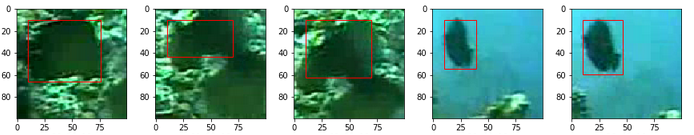
\includegraphics[scale=0.4]{image/sample.png}
\caption{Sample frames of the dataset}
\end{figure}

\end{frame}



\begin{frame}
\frametitle{Background - Cleaning Algorithm}

\begin{columns}
\column{0.59\textwidth}
\begin{itemize}
\item
The project uses the cleaning algorithm, the Pipeline Classifier developed by Matthew Pugh\cite{Pugh}. 
\item
The majority of the project's challenge came from the translation and optimization of the pipeline, as this classifier is still at experimental stage.
\item
For example, the SQL server is not used due to the limit of resources.
And the CNN part is abandoned due to mistakes during previous training stages.
\end{itemize}

\column{0.41\textwidth}
\begin{figure}
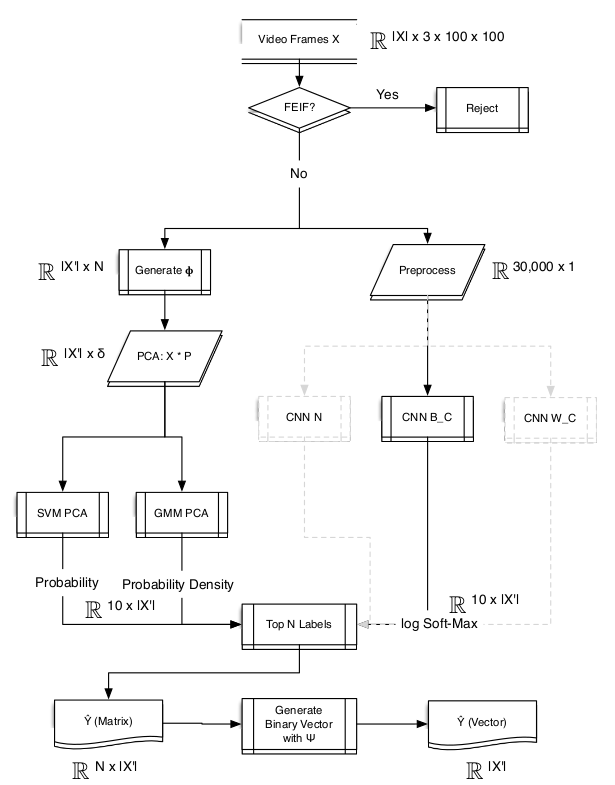
\includegraphics[scale=0.2]{image/pipe.png}
\caption{Pipeline Classifier}
\end{figure}
\end{columns}

\end{frame}



\subsection{Outcomes}

\begin{frame}
\frametitle{Project Outcomes}

The project has made following contribution on cleaning the dataset:
\begin{itemize}
\item
Using standard I/O stream script to extract data from SQL dump file, removes the cost of maintain a server.
\item
Translated most part of the Pipeline Classifier into Python.
\item
A MPI application distributing tasks over 200 DICE machines.
\item
Attempts on voting strategy to utilize classifier results.
\end{itemize}
\vspace{10pt}
The final cleaning removes 40\% of the False Positives at the cost of 10\% of True Positive. This reduces the Dataset by 28\%.

\end{frame}



\section{Details of Problems and Solution}
\subsection{Parallel Distribution}

\begin{frame}
\frametitle{Details - Parallel Distribution}

The first challenge is the distribution of the task.
\begin{itemize}
\item
This project uses the student lab DICE machines in Appleton Tower for the cleaning algorithm.
\item
There are 350 DICE machines in total. Due to auto-sleeping setting of some machines, about 220 can be used for cleaning.
\item
A Python script is used to ``scan'' for idle machines so the cleaning won't disrupt other students.
\item
With the shared file system - AFS, the more portable MPI is used for the project. This gives fast communication between the cleaning processes, hence achieves the demand of task distribution.
\end{itemize}

\end{frame}



\subsection{Data Extraction from SQL dump file}

\begin{frame}
\frametitle{Details - Standard I/O Stream Extraction}

Another problem of the project is the lack of a SQL server.
\begin{itemize}
\item
The F4K project's dataset contains a 500 GB {\tt .sql} dump file.
\item
Computing Support recommends me not to load the dump file using school's PostgreSQL service.
\item
Since the records needed are independent, it's possible to partition the data into csv file with a standard I/O pipeline.
\item
After parsing, loading relevant information of a 2000-frame video from AFS took less than 1 seconds now.
\item
It also gives more portability to the project.
\end{itemize}

\end{frame}



\subsection{Code Translation}

\begin{frame}
\frametitle{Details - Translating MATLAB code into Python}

Originally, one of the main goal is to translate the Pipeline Classifier into Python.

\begin{columns}
\column{0.59\textwidth}
\begin{itemize}
\item
The project have translated most of the parts into Python.
\item
Except for the Feature Extraction in MATLAB and the Neural Network in Lua.
\item
After some benchmarking it is estimated the translation could take more time than running the code directly.
\item 
PyMatlab and Lutorpy library is used to call the untranslated functions.
\end{itemize}

\column{0.41\textwidth}
\begin{figure}
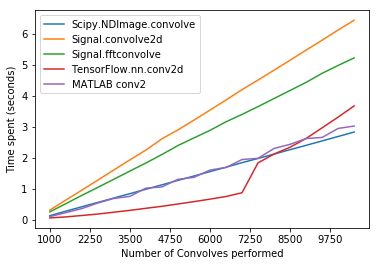
\includegraphics[scale=0.3]{image/benchmark.png}
\caption{Performance of different convolution algorithms}
\end{figure}
\end{columns}

\end{frame}



\subsection{Ground Truthing Dataset}

\begin{frame}
\frametitle{Details - Ground Truth}

In order to train the classifiers used in the pipeline, Pugh marked 60,000 detections manually using a 10-class classification schema.

\vspace{5pt}
In this schema, only class 6 and 8 are accepted fishes, while others will be rejected from the dataset.

\begin{figure}
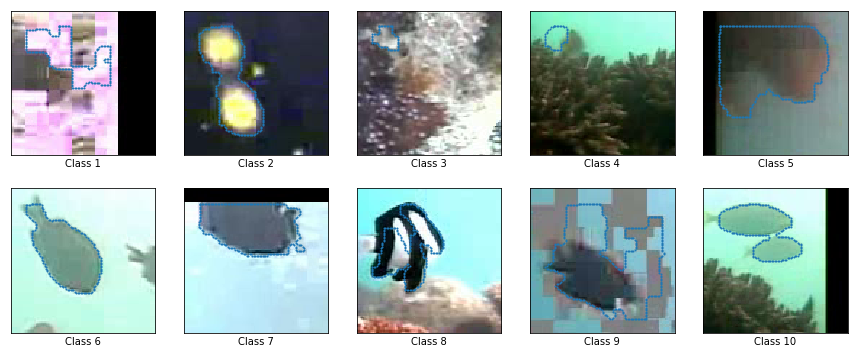
\includegraphics[scale=0.2]{image/class_sample.png}
\caption{Sample fish from each class}
\end{figure}

\vspace{-15pt}
Another 20,000 detections are marked in this project for complementing the missing cases, and performance evaluation.

\end{frame}



\subsection{Classifiers}

\begin{frame}
\frametitle{Details - Classifiers}

Pugh's pipeline classifier uses Support Vector Machine (SVM) and Convolutional Neural Network (CNN) for the classification of fish detections.

\begin{itemize}
\item
The SVM performed the same as Pugh's expectation.
\item
Unfortunately, the CNNs trained does not work as intended.
This is caused by color space issues in OpenCV. This leads to wrong transformation and normalization of the color spaces.
\item
Retraining the CNN would take a long time due to DICE machine's lack of CUDA support.
\end{itemize}

\begin{columns}
\setlength{\abovecaptionskip}{-2pt}
\column{0.5\textwidth}
\begin{figure}
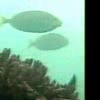
\includegraphics[scale=0.6]{image/outfile.jpg}
\caption{Normal Image in RGB space}
\end{figure}

\column{0.6\textwidth}
\begin{figure}
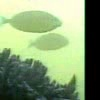
\includegraphics[scale=0.6]{image/outfile2.jpg}
\caption{OpenCV output, in BGR space}
\end{figure}
\end{columns}

\end{frame}



\subsection{Voting Strategy}

\begin{frame}
\frametitle{Details - Voting Strategy}

Even after the CNN failure mentioned above, the CNN might still be useful. As it's giving 80\% accuracy on class 6 (Fish) prediction. 

\vspace{5pt}
In order to utilizing the result from CNN, an attempt of voting strategy using the classifier outputs were made.

\vspace{8pt}
\begin{columns}
\column{0.5\textwidth}
To show the relationship between True/False Positive Rate, the ROC curve of different strategies are plotted.

\vspace{5pt}
With the need of keeping most of True Positives, the best strategy is using SVM results only.
\column{0.4\textwidth}
\begin{figure}
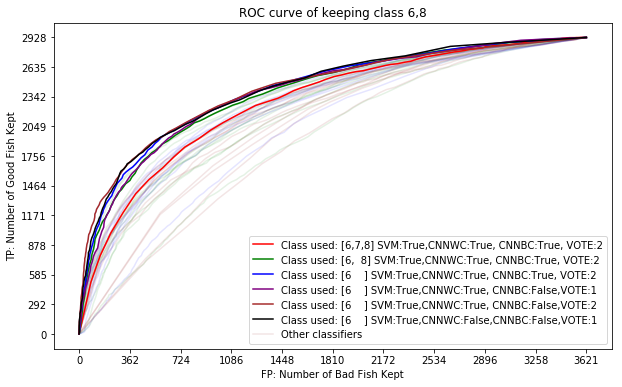
\includegraphics[scale=0.2]{image/roccurve.png}
\end{figure}
\end{columns}
\end{frame}



\section{Results}
\subsection{Project Result}
\begin{frame}
\frametitle{Result - Outcome}

The project manages to apply the cleaning algorithm developed by Pugh, with following statistics:
\begin{itemize}
\item
28\% of the 1.6 TB dataset is removed.
\item
40\% of the False Positive is marked as Non-Fish.
\item
Finished the task in 11 days of computational time.
\end{itemize}
\end{frame}



\subsection{Project Result}
\begin{frame}
\frametitle{Result - Sample True Positive/ False Positive}

\(<\)insert samples here\(>\)

\(<\)Forum power down - need access to project space to add images\(>\)

\end{frame}



\section{Conclusion}
\subsection{Lessons Learned}
\begin{frame}
\frametitle{Lessons Learned}
\end{frame}

\subsection{Future Work}
\begin{frame}
\frametitle{Future Work}
\end{frame}



\section*{Bibliography}
\setbeamertemplate{bibliography item}{\insertbiblabel}
\begin{frame}
\frametitle{Bibliography}
\begin{thebibliography}{3} % Beamer does not support BibTeX so references must be inserted manually as below
\bibitem{Pugh}
Matthew Pugh.
\newblock Removing false detections from a large fish image data-set.
\newblock Msc dissertation, The University of Edinburgh, 2015.

\bibitem{Yu}
Qiqi Yu.
\newblock Adding temporal constraints to a large data cleaning problem.
\newblock Msc dissertation, The University of Edinburgh, 2016.

\bibitem{F4K}
Robert B Fisher{,} Yun-Heh Chen-Burger{,} Daniela Giordano{,} Lynda Hardman{,}
  Fang-Pang Lin.
\newblock {\em Fish4Knowledge: collecting and analyzing massive coral reef fish
  video data}.
\newblock Springer, 2016.

\end{thebibliography}
\end{frame}

\end{document}